% !TeX root = chapter3_2d_ixaru.tex
% !TeX root = thesis.tex
\ifdefined\UtilIncluded
  \renewcommand{\startchapter}[1]{}
  \renewcommand{\stopchapter}{}
  \renewcommand{\undefinedlabel}[2]{}
\else

\newcommand{\startchapter}[1]{\begin{document}\setcounter{chapter}{#1}\addtocounter{chapter}{-1}}
\newcommand{\stopchapter}{\printbibliography[title=Bibliography,heading=bibintoc]\end{document}}


\documentclass{book}
\usepackage[utf8]{inputenc}


\usepackage{geometry}
\geometry{
  papersize={170mm,240mm},
}

\usepackage{amsfonts,amsmath, amsthm, amssymb, mathtools}
\usepackage{xspace}
\usepackage[hidelinks,bookmarks,pdfusetitle]{hyperref}
\usepackage{listings}
\usepackage[pdftex]{graphicx}
\usepackage{bm}
\usepackage[english]{babel}
\usepackage{caption}
\usepackage{subcaption}
\usepackage[usenames,dvipsnames]{xcolor}
\usepackage{physics}
\usepackage{multicol}
\usepackage{xstring}
\usepackage{pythonhighlight}
\usepackage{parskip}
\usepackage{thmtools}
\usepackage{relsize}
\usepackage{bookmark}
\usepackage{lmodern}
\usepackage{ifthen}
\usepackage{biblatex}
\usepackage{microtype}
\usepackage{csquotes}
\usepackage{numprint}
\usepackage{mleftright}
\npthousandsep{{\ifmmode\mskip2mu\else\hskip0.2em\fi}}
\npdecimalsign{.}

\addbibresource{references.bib}

\newtheorem{theorem}{Theorem}[chapter]
\newtheorem{lemma}[theorem]{Lemma}
\newtheorem{corollary}[theorem]{Corollary}
\newtheorem{definition}[theorem]{Definition}

\DeclareRobustCommand{\oneD}{{1{\relsize{-1}D}}\xspace}
\DeclareRobustCommand{\twoD}{{2{\relsize{-1}D}}\xspace}
\DeclareRobustCommand{\threeD}{{3{\relsize{-1}D}}\xspace}
\DeclareRobustCommand{\cpp}{{{C\nolinebreak[4]\hspace{-.05em}\raisebox{.4ex}{\relsize{-3}\textbf{++}}}\xspace}}
\pdfstringdefDisableCommands{%
  \def\cpp{C++}%
  \def\oneD{1D}%
  \def\twoD{2D}%
  \def\threeD{3D}%
}

\newcommand{\longchapter}[2][]{%
  \chapter[#2]{#2}%
  \ifthenelse{\equal{#1}{}}{}{\chaptermark{#1}}}

\newcommand{\NN}{\mathbb{N}}
\newcommand{\ZZ}{\mathbb{Z}}
\newcommand{\QQ}{\mathbb{Q}}
\newcommand{\QQbar}{\overline{\mathbb{Q}}}
\newcommand{\RR}{\mathbb{R}}
\newcommand{\CC}{\mathbb{C}}

\newcommand{\Eigen}{\texttt{Eigen}}

\newcommand{\sage}{\texttt{sage}\xspace}

\newcommand{\hamiltonian}{\mathcal{H}}

\newcommand{\transposesign}{\intercal}
\newcommand{\transpose}[1]{{#1}^\transposesign}
\newcommand{\adjointsign}{\text{H}}
\newcommand{\adjoint}[1]{{#1}^\adjointsign}

\newcommand{\xmin}{{x_{\text{min}}}}
\newcommand{\xmax}{{x_{\text{max}}}}
\newcommand{\ymin}{{y_{\text{min}}}}
\newcommand{\ymax}{{y_{\text{max}}}}

\newcommand{\Cbottom}{\vb{C}_\text{bottom}}
\newcommand{\Ctop}{\vb{C}_\text{top}}
\newcommand{\ubottom}{\vb{u}_\text{bottom}}
\newcommand{\utop}{\vb{u}_\text{top}}

\DeclareMathOperator{\diag}{diag}
\DeclareMathOperator{\tridiag}{tridiag}
\DeclareMathOperator{\eigs}{eigs}
\DeclareMathOperator*{\argmin}{arg\,min}
\DeclareMathOperator{\Ai}{Ai}
\DeclareMathOperator{\Bi}{Bi}
\DeclareMathOperator{\OO}{\mathcal{O}}

% https://tex.stackexchange.com/a/18192/163747
\makeatletter
\newcommand{\undefinedlabel}[2]{%
  \protected@write \@auxout {}{\string \newlabel {#1}{{#2}{\thepage}{#2}{#1}{}} }%
  \hypertarget{#1}{}
}
\makeatother

\fi
\gdef\UtilIncluded{}


\startchapter{3}

\undefinedlabel{sec:c1_selfadjoint}{1.-}

\longchapter[A shooting method]{A shooting method for the \twoD time-independent Schrödinger equation}

There are many general methods for partial differential equations. Each method has its own benefits and disadvantages. As a rule of thumb one can say that a method which is very general and widely applicable, will be less efficient, less accurate or both then a method which is specifically tuned for the problem at hand. With that in mind, there is a real advantage to gain when investing time and research into a highly tuned optimized method for a specific problem.

In this, and the next, chapter we will study two-dimensional time-independent Schrödinger equations
\begin{equation}\label{equ:c3_schrodinger_2d}
    -\nabla^2\psi(x, y) + V(x, y) \psi(x, y) = \lambda \psi(x, y)
\end{equation}
on the domain $\Omega = [\xmin, \xmax]\times[\ymin, \ymax]$. We will only consider homogenous Dirichlet boundary conditions, this means $\forall (x, y) \in \delta\Omega : \psi(x, y) = 0$. The function $V: \RR^2 \to \RR$ is called the potential function. This potential, together with the domain, defines the Schrödinger problem. When \emph{solving} the time-independent Schrödinger equation, one is searching for values for $\lambda$ such that a function $\psi(x, y)$  exists such they together satisfy the equation \eqref{equ:c3_schrodinger_2d}. Such a value $\lambda$ is called an \emph{eigenvalue} with the corresponding \emph{eigenfunction} $\psi(x, y)$.

Equation \eqref{equ:c3_schrodinger_2d} can also be interpreted as finding the eigenvalues and eigenfunctions of the \emph{Hamiltonian} $\hamiltonian$:
$$
    \hamiltonian := -\nabla^2 + V(x, y)\text{.}
$$
\begin{theorem}
    The Hamiltonian operator with homogenous Dirichlet boundary conditions is self-adjoint. And some more adjectives.
\end{theorem}
\begin{proof}
    To prove that $H$ is self-adjoint, it is sufficient to prove that $\bra{\hamiltonian f}\ket{g} = \bra{f}\ket{\hamiltonian g}$, for functions $f$ and $g$ {\color{red} To do: which function space?}. This can be shown by direct computation.
    \begin{align*}
        \bra{\hamiltonian f}\ket{g} & = \int_\Omega \hamiltonian f g                                                                                                        \\
                                    & = -\int_\Omega \nabla^2 f g + \int_\Omega V f g                                                                                       \\
        \intertext{Applying Green's second identity yields the following. Here $\vb{n}$ is the outward pointing surface normal of $\dd S$ }
                                    & = -\int_\Omega f \nabla^2 g + \oint_{\delta\Omega} \left( f \pdv[]{g}{\vb{n}} - \pdv[]{f}{\vb{n}} g  \right)\dd S + \int_\Omega V f g \\
        \intertext{Recalling the homogenous Dirichlet boundary conditions, allows us to remove the second term, as $f(x,y) = g(x, y) = 0$ for all $(x, y) \in \delta\Omega$.}
                                    & =\int_\Omega f\,\left(-\nabla^2 g  + V g\right)                                                                                       \\
                                    & = \bra{f}\ket{\hamiltonian g}
    \end{align*}
\end{proof}

Proving the Hamiltonian is a linear self-adjoint operator allows us to employ the theory as described in section \ref{sec:c1_selfadjoint}. In particular, we now know that the eigenvalues of $\hamiltonian$ or real, and if $\Omega$ is bounded, the spectrum is discrete and countable. Furthermore, the eigenfunctions are orthogonal.

For almost all potential functions $V$ the corresponding Schrödinger equation can not be solved symbolically. So when you are interested in solutions, you will have to resort to numerical methods. When only the ground state, that is the lowest eigenvalue, or maybe only few of the lowest eigenvalues are required, general numerical methods may suffice. Some examples of such techniques are finite difference based methods, or a finite element analysis. When higher eigenvalues are required, the eigenfunctions become more and more oscillatory, and as such, harder to find.

In \cite{ixaru_new_2010} a new method is proposed to approximate solutions of the two-dimensional time-independent Schrödinger equations.

\section{Ixaru's method}

 {\color{red} To do: this is a direct copy from the article: proofread}

The main idea of Ixaru's method is built on the well established technique \cite{titchmarsh_eigenfunction_1962} of writing a solution as a linear combination of well-chosen one dimensional basis functions $b_i(x)$: $\psi(x, y) = \sum_{i=1}^\infty b_i(x) c_i(y)$. A disadvantage of this known technique is that very many basis functions are necessary to ensure accurate solutions. Ixaru mitigates this by proposing multiple sets of basis functions, depending on the position in the domain. More concretely he suggests splitting the domain into $K$ different sectors along the $y$-axis\footnote{In the original article \cite{ixaru_new_2010} Ixaru splits the domain along the $x$-axis. But for notational purposes it is more natural to split along the $y$-axis. Analogous for the 3d version of the method, the split would happen along the $z$-axis.}:
$$
    \ymin = y_0 < y_1 < y_2 < \dots < y_k < \dots < y_{K-1} < y_{K} = \ymax\text{.}
$$
This split in sectors is illustrated in figure \ref{fig:c3_2dsectors}.

\begin{figure}
    \begin{center}
        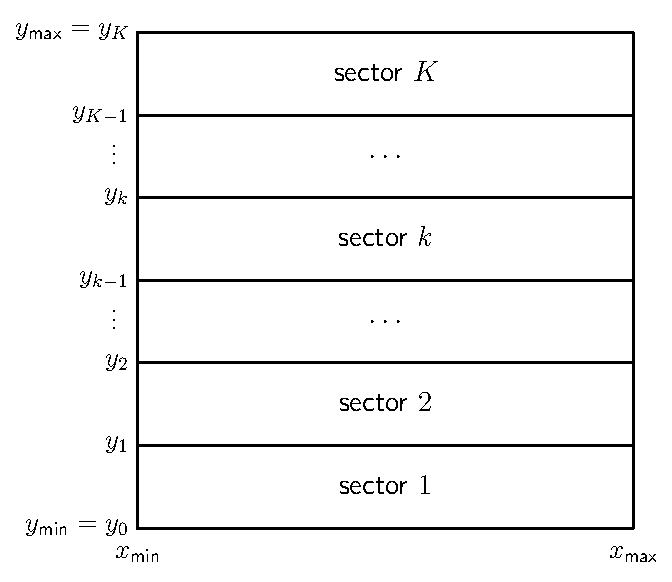
\includegraphics[width=.6\textwidth]{img/chapter3/2dsectors.pdf}
        \caption{\label{fig:c3_2dsectors} An illustration of the split in sectors along the $y$-axis for the domain $[\xmin, \xmax]\times[\ymin, \ymax]$.}
    \end{center}
\end{figure}

On each sector $k$ (with domain $[\xmin, \xmax]\times[y_{k-1}, y_k]$) a solution $\psi(x, y)$ will be approximated as a linear combination of the first $N$ basis functions:
\begin{equation}\label{equ:c3_lincomb_basis}
    \psi(x, y) \approx \sum_{i=1}^{N} b_i^{(k)}(x) c_i^{(k)}(y) = \transpose{\vb{b}^{(k)}}(x) \, \vb{c}^{(k)}(y) \text{.}
\end{equation}

The well-chosen basis $\left\{b_i^{(k)}\right\}$ Ixaru proposes can be calculated from the one dimensional Schrödinger equation. Let $b_i^{(k)}(x)$ be defined as the $i^\text{th}$ eigenfunction of the eigenvalue problem
$$
    -\pdv[2]{b_i^{(k)}}{x} + \bar{V}^{(k)}(x)b_i^{(k)}(x) = \lambda_i^{(k)} b_i^{(k)}(x)
$$
with boundary conditions $b_i^{(k)}(\xmin) = b_i^{(k)}(\xmax) = 0$. The function $\bar{V}^{(k)}(x)$ is a constant (in the $y$-direction) approximation of the potential $V$ on the $k^\text{th}$ sector. Ixaru proposes $\bar{V}^{(k)}(x) := V\left(x, \frac{y_{k-1} + y_k}{2}\right)$, we will later remark that other choices can be defended as well.

Just like the CP-methods, this new method employs shooting to locate the eigenvalues. For this, for a fixed value of $E$, formulae are needed to propagate solutions from the bottom of the domain (along $y = \ymin$) upwards, and from the top of the domain ($y = \ymax$) downwards. So, given a solution at the beginning of sector $k$ expressed in the basis $b_i^{(k)}$:
$ \psi(x, y_{k-1}) = \sum_{i=1}^{N} b_i^{(k)}(x)\, c_i^{(k)}(y_{k-1}) $, an expression is constructed to compute $c^{(k)}_i(y_k)$ at the end of the sector. Substituting \eqref{equ:c3_lincomb_basis} into \eqref{equ:c3_schrodinger_2d} gives rise to

\begin{equation}\label{equ:c3_coupled_system}
    -\pdv[2]{\vb{c}^{(k)}}{y} + \vb{V}^{(k)}(y) \vb{c}^{(k)}(y) = E \vb{c}^{(k)}(y) \text{.}
\end{equation}

In this expression $\vb{V}^{(k)}$ is an $N\times N$ matrix dependent on $y$:
\begin{equation}\label{equ:c3_v_matrix}
    \vb{V}^{(k)}_{ij}(y) = \int_{\xmin}^{\xmax} b_i^{(k)}(x) b_j^{(k)}(x) \left(V(x, y) - \bar{V}^{(k)}(x)\right) \dd x + \delta_{ij} \lambda_i^{(k)} \text{.}
\end{equation}

The system of ordinary differential equations given in \eqref{equ:c3_coupled_system} is a coupled system of Schrö\-dinger equations. For coupled systems, there are well-known CP-methods available \cite{ledoux_numerical_2007a,ixaru_lilix_2002a}, with various implementations.

For the accurate computation of the integral in \eqref{equ:c3_v_matrix} we have developed specialized formulae. These will be presented later on in section \ref{sec:c3_calculate_vk}.

To be able to propagate a solution along the whole domain it is vital to have an expression to transfer solutions between consecutive sectors. To have continuous and continuously differentiable solutions, this property should also exist on the transition line between sectors. Therefore,
\begin{align*}
    \transpose{\vb{b}^{(k)}}(x) \, \vb{c}^{(k)}(y_k)                   & =\, \transpose{\vb{b}^{(k+1)}}(x) \, \vb{c}^{(k+1)}(y_k)                   \\
    \text{and}\quad
    \transpose{\vb{b}^{(k)}}(x)\,\pdv{\vb{c}^{(k)}}{y}\left(y_k\right) & = \transpose{\vb{b}^{(k+1)}}(x)\,\pdv[]{\vb{c}^{(k+1)}}{y}\left(y_k\right)
\end{align*}
should hold for all values of $x$. Multiplying both sides with $b_i^{(k)}$ and integrating along the $x$-axis for each $i \in \{1, \dots, N\}$, gives
\begin{align*}
    \vb{c}^{(k+1)}(y_k)                       & = \vb{M}^{(k)} \vb{c}^{(k)}(y_k)                       \\
    \pdv[]{\vb{c}^{(k+1)}}{y}\left(y_k\right) & = \vb{M}^{(k)} \pdv[]{\vb{c}^{(k)}}{y}\left(y_k\right)
\end{align*}
with
$$
    \vb{M}^{(k)}_{ij} = \bra{b_{i}^{(k)}}\ket{b_{j}^{(k+1)}} = \int_\xmin^\xmax b_i^{(k)}(x) b_j^{(k+1)}(x) \dd x \text{.}
$$
This is in the assumption that the orthogonal basis $\left\{b_i^{(k)}(x)\right\}$ is normalized $\bra{b_{i}^{(k)}}\ket{b_{j}^{(k)}} = \delta_{ij}$. In the infinite case this matrix $\vb{M}^{(k)}$ is orthogonal. In practice $N$ has to be finite, and $\vb{M}^{(k)}$ is in general no longer orthogonal. Intuitively this means that some information about the solution is lost when transitioning between sectors. This is a minor drawback, inherent to this method.

With these tools available, all that is left is to formalize how the shooting can be executed. Instead of propagating with a single starting condition (i.e. a column vector $\vb{c}^{1}(\ymin)$) all possible initial values (for vanishing boundary conditions) are propagated at once.
$$
    \begin{matrix}
        \vb{C}^{(1)}(\ymin) = \vb{0}_{N\times N} &            & \pdv[]{\vb{C}^{(1)}}{y}\left(\ymin\right) = \vb{I}_{N\times N} \\
                                                 & \text{and} &                                                                \\
        \vb{C}^{(K)}(\ymax) = \vb{0}_{N\times N} &            & \pdv[]{\vb{C}^{(K)}}{y}\left(\ymax\right) = \vb{I}_{N\times N}
    \end{matrix}
$$

In the matching point $y_m$, solutions are found. Since solutions have to be continuous and continuously differentiable, a `matching' condition can be formulated.  Let us define $\Cbottom$ and $\Cbottom'$ to be the values of $\vb{c}^{(m)}(y_m)$ and $\pdv[]{\vb{c}^{(m)}}{y}\left(y_m\right)$ respectively when propagated from the bottom of the domain upwards. Analogous $\Ctop$ and $\Ctop'$ can be defined. Now the value $E$ is an eigenvalue of the original problem if and only if there exists vectors $\ubottom$ and $\utop$ such that
\begin{align*}
    \Cbottom \cdot \ubottom                   & = \Ctop \cdot \utop           \\
    \text{and }\quad \Cbottom' \cdot \ubottom & = \Ctop' \cdot \utop \text{.}
\end{align*}
This is equivalent with saying $E$ is an eigenvalue of \eqref{equ:c3_schrodinger_2d} if and only if the mismatch matrix
\begin{equation}\label{equ:c3_psi_e}
    \vb{\Phi}(E) := \Cbottom'\Cbottom^{-1} - \Ctop'\Ctop^{-1}
\end{equation}
has a zero eigenvalue. Note that the multiplicity of the zero eigenvalue of this matrix is the same as the multiplicity of $E$ as an eigenvalue of \eqref{equ:c3_schrodinger_2d}. In the original article no details are given about how one should find the values of $E$ for which the matrix $\vb{\Phi}(E)$ becomes singular. Later, in section \ref{sec:c3_locating_e}, we will present our method for finding those values. In section \ref{sec:c3_index_of_e}, we will go even further and demonstrate a technique which allows to determine the index of the eigenvalue in question.

This concludes our overview of the method described by Ixaru in \cite{ixaru_new_2010}. There are a few differences between our overview and the method as described in \cite{ixaru_new_2010}. Most notably, as stated in the beginning, we have swapped the roles of $x$ and $y$. Ixaru split the domain in sectors along the $x$-axis, while we think it is more natural to apply the split along the $y$-axis\footnote{The main reason for this change in notation is to make the recursive nature of this method apparent. In future work we use this method to also solve the 3d time-independent Schrödinger equation. For this we split the domain along the $z$-axis, and solve on each sector the 2d Schrödinger equation in the $x\,y$-plane. For each of these 2d equations we split the domain along the $y$-axis, and solve the one dimensional Schrödinger equation along the $x$-axis.}. But this difference is only notational and does not change anything fundamental about the method.

\section{Our improvements}

\subsection{Locating eigenvalues}\label{sec:c3_locating_e}

\subsection{Determining the index of an eigenvalue}\label{sec:c3_index_of_e}

\subsection{Calculation of \texorpdfstring{$\vb{V}^{(k)}(y)$}{Vk(y)}}\label{sec:c3_calculate_vk}


\section{Determining the index of eigenvalues}

\subsection{A test on a more exotic domain}


\begin{figure}
    \begin{center}
        \begin{minipage}{.5\textwidth}
            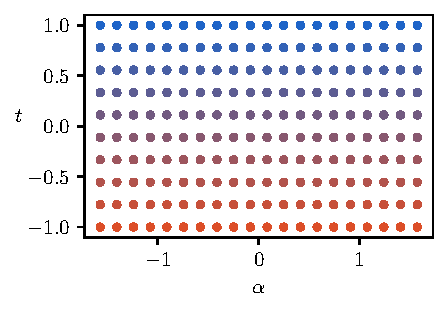
\includegraphics[width=\textwidth]{img/chapter3/on_disc/disc_original.pdf}%
        \end{minipage}\begin{minipage}{.1\textwidth}
            $$ \to $$
        \end{minipage}\begin{minipage}{.4\textwidth}
            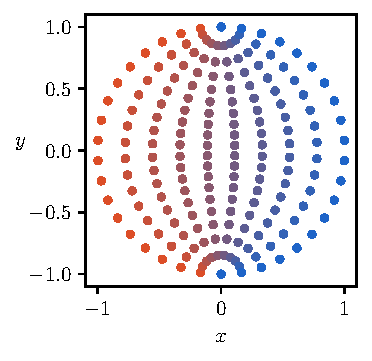
\includegraphics[width=\textwidth]{img/chapter3/on_disc/disc_transformed.pdf}
        \end{minipage}
    \end{center}
\end{figure}




\stopchapter
